\PassOptionsToPackage{dvipsnames}{xcolor}
\documentclass[english, a4paper,12pt]{article}
\usepackage[a4paper, top=2cm, bottom=2cm,right=2cm,left=2cm]{geometry}
\date{} 
\usepackage[utf8]{vietnam}
\usepackage{textcomp, graphicx, titling, tkz-tab, changepage}
\usepackage{changepage, amsmath, fancyvrb, minted, caption} 
\usepackage{booktabs}
\usepackage{tabularx}
\usepackage[dvipsnames]{xcolor}
\usepackage[english]{babel}
\usepackage{hyperref}
\hypersetup{
    colorlinks=true,
    linkcolor=black,
    filecolor=magenta,      
    urlcolor=Green,
    pdftitle={Overleaf Example},
    pdfpagemode=FullScreen,
    }
\addto\captionsenglish{
  \renewcommand{\contentsname}
  {Table of Contents}
}

\begin{document}
\begin{titlepage}
\begin{center}
\textbf{UNIVERSITY OF INFORMATION TECHNOLOGY}

\textbf{FACULTY OF COMPUTER SCIENCE}

\vspace{1cm}

\vspace{1cm}

\textbf{EVALUATION FUNCTIONS FOR MINIMAX/ALPHABETA/EXPECTIMAX}

\vspace{2cm}

\includegraphics[width= 5cm]{logo.png}
\vspace{2cm}

\textbf{Instructor: } Luong Ngoc Hoang

\vspace{0.5cm}

\textbf{Student:} Ha Huy Hoang - 22520460
\vspace{0.5cm}
\\
\textbf{Class:} CS106.O21
\vspace{2cm}
\tableofcontents
\end{center}
\end{titlepage}

\section*{1. Introduction}
\addcontentsline{toc}{section}{1. Introduction}
\hspace*{7mm}Pacman is an engaging game where the player navigates a Pacman character through a maze filled with food, capsules, and ghosts. The primary objective is to guide Pacman to consume all the capsules without getting trapped by the ghosts. By employing Adversarial and Random Search techniques, we can optimize the game strategy to achieve the highest possible score and ensure Pacman’s victory in this task. This approach allows us to anticipate the ghosts’ movements and make the most effective decisions for Pacman.
\begin{figure}[h]
\centering
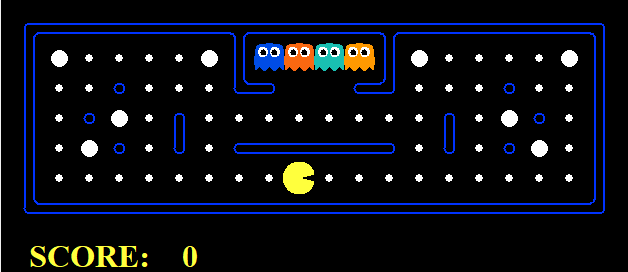
\includegraphics[width=10cm]{image.png}
\caption*{\textbf{Image 1.} An example map in Pacman}
\end{figure}
\section*{2. Idea of betterEvaluationFunction}
\addcontentsline{toc}{section}{2. Idea of betterEvaluationFunction}
\normalsize\hspace*{7mm}Evaluating Pacman’s intermediate states based solely on the score may not yield the most effective results. In this discussion, I will explore an approach that evaluates each element separately, such as the score, Pacman’s proximity to food, and his distance from ghosts, among others.
\vspace*{3mm}\\
\normalsize\hspace*{7mm}I will assign a reward value to each feature, and then calculate the score for each step taken towards the nearest object. Specifically we will have four main weights, as follows:
\begin{itemize}
\item eatenWeight = 300 (Award much more points to prioritize eating ghosts over food or capsules)
\item ghostWeight = 20 (Award additional points to prioritize avoiding ghosts over eating food or capsules)
\item foodWeight = 10 
 \item numWeight = 500 
\end{itemize}
\normalsize\hspace*{7mm}The function will evaluate the state through the weights and the number of steps Pacman moves to each corresponding object. We will take \textbf{score = currentGameState.getScore()} as the standard.
\\
\normalsize\hspace*{7mm}First, we will iterate through all the ghosts. If a ghost is in the \textbf{scaredTimer}, we will add to the score at that state \textbf{eatenWeight} divided by the number of steps Pacman takes to that ghost. If the ghost is not in a scared state, we will check if it is the closest ghost to Pacman. If it is, we subtract \textbf{ghostWeight} divided by the number of steps Pacman takes to it from the score, if the number of steps is greater than 0. If it equals 0, we subtract -99999999 points
\\
\hspace*{7mm}Second, we iterate through the Foods and Capsules, adding to the score an additional \textbf{foodWeight} divided by the number of steps to the nearest food or Capsule.
\\
\hspace*{7mm}Third, we add to the score an additional \textbf{numWeight} divided by the number of remaining food (the fewer the remaining food, the more points are added).

\section*{3. Statistics}
\addcontentsline{toc}{section}{3. Statistics}
\normalsize\hspace*{7mm}For convenience in statistics, I have written a file called \textbf{run\_for\_statistic.py}. Due to the limited configuration conditions of my computer, I can only run a maximum of \textbf{‘depth = 3’}. Specifically, the trickyClassic, openClassic, and originalClassic levels can only run \textbf{‘depth = 2’}.
\vspace*{3mm}\\
\normalsize\hspace*{7mm}In the case of openClassic, because the eval function uses scoreEvaluationFunction, it only estimates based on the score and I can only evaluate within 2 steps. Therefore, Pacman just stands and moves around a corner. So, if using scoreEvaluationFunction in this level, the score would be \textbf{-} (undefiend)
\vspace*{3mm}\\
\hspace*{7mm} This is \href{https://drive.google.com/file/d/1NlazYIF-0y74FMNw7oUwt-5tSI75wtdM/view?usp=sharing}{the best result video} I could achieve when running the mediumClassic layout with Expectimax, betterEvaluationFunction, and depth = 3.
\subsection*{capsuleClassic.lay, depth = 3}
\small\begin{tabular}{|c|c|c|c|c|c|c|}
\hline
{\textbf{RandomSeed}}& \multicolumn{3}{c|}{\textbf{scoreEvaluationFunction}} & \multicolumn{3}{c|}{\textbf{betterEvaluationFunction}} \\
\cline{2-7}
& \textbf{Minimax} & \textbf{AlphaBeta} & \textbf{Expectimax} & \textbf{Minimax} & \textbf{AlphaBeta} & \textbf{Expectimax} \\
\hline
22520460 & \textcolor{red!70}{-438}& \textcolor{red!70}{-438} & \textcolor{red!70}{-187} & \textcolor{red!70}{-66} & \textcolor{red!70}{-66} & \textcolor{Green}{972} \\
22520461 & \textcolor{red!70}{-457} & \textcolor{red!70}{-457} & \textcolor{red!70}{-458} & \textcolor{red!70}{-13} & \textcolor{red!70}{-13} & \textcolor{red!70}{783} \\
22520462 & \textcolor{red!70}{-431} & \textcolor{red!70}{-431} & \textcolor{red!70}{-431} & \textcolor{red!70}{-431} & \textcolor{red!70}{-431} & \textcolor{red!70}{-430} \\
22520463 & \textcolor{red!70}{-587} & \textcolor{red!70}{-587} & \textcolor{red!70}{-44} & \textcolor{red!70}{789} & \textcolor{red!70}{789} & \textcolor{red!70}{796} \\
22520464 & \textcolor{red!70}{-448} & \textcolor{red!70}{-448} & \textcolor{red!70}{-232} & \textcolor{Green}{804} & \textcolor{Green}{804} & \textcolor{Green}{1192} \\
\hline
\end{tabular}

\subsection*{contestClassic.lay, depth = 3}
\small\begin{tabular}{|c|c|c|c|c|c|c|}
\hline
\textbf{RandomSeed} & \multicolumn{3}{c|}{\textbf{scoreEvaluationFunction}} & \multicolumn{3}{c|}{\textbf{betterEvaluationFunction}} \\
\cline{2-7}
& \textbf{Minimax} & \textbf{AlphaBeta} & \textbf{Expectimax} & \textbf{Minimax} & \textbf{AlphaBeta} & \textbf{Expectimax} \\
\hline
22520460 & \textcolor{red!70}{349} & \textcolor{red!70}{349} & \textcolor{red!70}{349} & \textcolor{red!70}{2290} & \textcolor{red!70}{2290} & \textcolor{red!70}{1840} \\
22520461 & \textcolor{red!70}{-21} & \textcolor{red!70}{-21} & \textcolor{red!70}{-21} & \textcolor{red!70}{1836} & \textcolor{red!70}{1836} & \textcolor{red!70}{1534} \\
22520462 & \textcolor{red!70}{-39} & \textcolor{red!70}{-39} & \textcolor{red!70}{908} & \textcolor{Green}{3153} & \textcolor{Green}{3153} & \textcolor{red!70}{931} \\
22520463 & \textcolor{red!70}{63} & \textcolor{red!70}{63} & \textcolor{red!70}{1732} & \textcolor{red!70}{1460} & \textcolor{red!70}{1460} & \textcolor{Green}{2997} \\
22520464 & \textcolor{red!70}{-124} & \textcolor{red!70}{-124} & \textcolor{red!70}{1079} & \textcolor{red!70}{211} & \textcolor{red!70}{211} & \textcolor{Green}{2922} \\
\hline
\end{tabular}

\subsection*{mediumClassic.lay, depth = 3}
\small\begin{tabular}{|c|c|c|c|c|c|c|}
\hline
\textbf{RandomSeed} & \multicolumn{3}{c|}{\textbf{scoreEvaluationFunction}} & \multicolumn{3}{c|}{\textbf{betterEvaluationFunction}} \\
\cline{2-7}
& \textbf{Minimax} & \textbf{AlphaBeta} & \textbf{Expectimax} & \textbf{Minimax} & \textbf{AlphaBeta} & \textbf{Expectimax} \\
\hline
22520460 & \textcolor{red!70}{370} & \textcolor{red!70}{370} & \textcolor{red!70}{-2292} & \textcolor{Green}{1839} & \textcolor{Green}{1839} & \textcolor{Green}{2112} \\
22520461 & \textcolor{Green}{1313} & \textcolor{Green}{1313} & \textcolor{Green}{1313} & \textcolor{Green}{1869} & \textcolor{Green}{1869} & \textcolor{Green}{1634} \\
22520462 & \textcolor{Green}{1679} & \textcolor{Green}{1679} & \textcolor{Green}{1679} & \textcolor{Green}{2003} & \textcolor{Green}{2003} & \textcolor{Green}{1934} \\
22520463 & \textcolor{red!70}{-4339} & \textcolor{red!70}{-4339} & \textcolor{red!70}{-7284} & \textcolor{red!70}{913} & \textcolor{red!70}{913} & \textcolor{Green}{1923} \\
22520464 & \textcolor{red!70}{-1071} & \textcolor{red!70}{-1071} & \textcolor{red!70}{278} & \textcolor{Green}{2076} & \textcolor{Green}{2076} & \textcolor{Green}{2051} \\
\hline
\end{tabular}

\subsection*{minimaxClassic.lay, depth = 3}
\small\begin{tabular}{|c|c|c|c|c|c|c|}
\hline
\textbf{RandomSeed} & \multicolumn{3}{c|}{\textbf{scoreEvaluationFunction}} & \multicolumn{3}{c|}{\textbf{betterEvaluationFunction}} \\
\cline{2-7}
& \textbf{Minimax} & \textbf{AlphaBeta} & \textbf{Expectimax} & \textbf{Minimax} & \textbf{AlphaBeta} & \textbf{Expectimax} \\
\hline
22520460 & \textcolor{red!70}{-496} & \textcolor{red!70}{-496} & \textcolor{red!70}{-498} & \textcolor{red!70}{-496} & \textcolor{red!70}{-496} & \textcolor{red!70}{-498} \\
22520461 & \textcolor{Green}{509} & \textcolor{Green}{509} & \textcolor{Green}{513} & \textcolor{Green}{502} & \textcolor{Green}{502} & \textcolor{Green}{502} \\
22520462 & \textcolor{red!70}{-496} & \textcolor{red!70}{-496} & \textcolor{red!70}{-496} & \textcolor{red!70}{-496} & \textcolor{red!70}{-496} & \textcolor{red!70}{-497} \\
22520463 & \textcolor{Green}{514} & \textcolor{Green}{514} & \textcolor{Green}{515} & \textcolor{Green}{514} & \textcolor{Green}{514} & \textcolor{Green}{514} \\
22520464 & \textcolor{Green}{512} & \textcolor{Green}{512} & \textcolor{Green}{512} & \textcolor{red!70}{-498} & \textcolor{red!70}{-498} & \textcolor{Green}{509} \\
\hline
\end{tabular}

\subsection*{openClassic.lay, depth = 2}
\small\begin{tabular}{|c|c|c|c|c|c|c|}
\hline
\textbf{RandomSeed} & \multicolumn{3}{c|}{\textbf{scoreEvaluationFunction}} & \multicolumn{3}{c|}{\textbf{betterEvaluationFunction}} \\
\cline{2-7}
& \textbf{Minimax} & \textbf{AlphaBeta} & \textbf{Expectimax} & \textbf{Minimax} & \textbf{AlphaBeta} & \textbf{Expectimax} \\
\hline
22520460 & \textcolor{red!70}{-} & \textcolor{red!70}{-} & \textcolor{red!70}{-} & \textcolor{Green}{1157} & \textcolor{Green}{1157} & \textcolor{Green}{1293} \\
22520461 & \textcolor{Green}{-} & \textcolor{red!70}{-} & \textcolor{red!70}{-} & \textcolor{Green}{1416} & \textcolor{Green}{1416} & \textcolor{Green}{1056} \\
22520462 & \textcolor{red!70}{-} & \textcolor{red!70}{-} & \textcolor{red!70}{-} & \textcolor{Green}{1352} & \textcolor{Green}{1352} & \textcolor{Green}{1273} \\
22520463 & \textcolor{red!70}{-} & \textcolor{red!70}{-} & \textcolor{red!70}{-} & \textcolor{Green}{1217} & \textcolor{Green}{1217} & \textcolor{Green}{1230} \\
22520464 & \textcolor{red!70}{-} & \textcolor{red!70}{-} & \textcolor{red!70}{-} & \textcolor{Green}{1416} & \textcolor{Green}{1416} & \textcolor{Green}{1426} \\
\hline
\end{tabular}

\subsection*{originalClassic.lay, depth = 2}
\small\begin{tabular}{|c|c|c|c|c|c|c|}
\hline
\textbf{RandomSeed} & \multicolumn{3}{c|}{\textbf{scoreEvaluationFunction}} & \multicolumn{3}{c|}{\textbf{betterEvaluationFunction}} \\
\cline{2-7}
& \textbf{Minimax} & \textbf{AlphaBeta} & \textbf{Expectimax} & \textbf{Minimax} & \textbf{AlphaBeta} & \textbf{Expectimax} \\
\hline
22520460 & \textcolor{red!70}{325} & \textcolor{red!70}{325} & \textcolor{red!70}{325} & \textcolor{Green}{2479} & \textcolor{Green}{2479} & \textcolor{red!70}{1641} \\
22520461 & \textcolor{red!70}{364} & \textcolor{red!70}{364} & \textcolor{red!70}{488} & \textcolor{red!70}{-27} & \textcolor{red!70}{-27} & \textcolor{Green}{3277} \\
22520462 & \textcolor{red!70}{42} & \textcolor{red!70}{42} & \textcolor{red!70}{42} & \textcolor{red!70}{942} & \textcolor{red!70}{942} & \textcolor{Green}{2852} \\
22520463 & \textcolor{red!70}{71} & \textcolor{red!70}{71} & \textcolor{red!70}{71} & \textcolor{red!70}{855} & \textcolor{red!70}{855} & \textcolor{red!70}{2205} \\
22520464 & \textcolor{red!70}{-45} & \textcolor{red!70}{-45} & \textcolor{red!70}{-45} & \textcolor{red!70}{2094} & \textcolor{red!70}{2094} & \textcolor{Green}{2245} \\
\hline
\end{tabular}

\subsection*{powerClassic.lay, depth = 3}
\small\begin{tabular}{|c|c|c|c|c|c|c|}
\hline
\textbf{RandomSeed} & \multicolumn{3}{c|}{\textbf{scoreEvaluationFunction}} & \multicolumn{3}{c|}{\textbf{betterEvaluationFunction}} \\
\cline{2-7}
& \textbf{Minimax} & \textbf{AlphaBeta} & \textbf{Expectimax} & \textbf{Minimax} & \textbf{AlphaBeta} & \textbf{Expectimax} \\
\hline
22520460 & \textcolor{Green}{3190} & \textcolor{Green}{3190} & \textcolor{red!70}{472} & \textcolor{Green}{4528} & \textcolor{Green}{4528} & \textcolor{Green}{5801} \\
22520461 & \textcolor{Green}{3658} & \textcolor{Green}{3658} & \textcolor{Green}{2561} & \textcolor{red!70}{2077} & \textcolor{red!70}{2077} & \textcolor{red!70}{3560} \\
22520462 & \textcolor{Green}{2383} & \textcolor{Green}{2383} & \textcolor{Green}{3472} & \textcolor{Green}{4426} & \textcolor{Green}{4426} & \textcolor{red!70}{4059} \\
22520463 & \textcolor{red!70}{611} & \textcolor{red!70}{611} & \textcolor{red!70}{891} & \textcolor{Green}{960} & \textcolor{Green}{4960} & \textcolor{Green}{5228} \\
22520464 & \textcolor{red!70}{998} & \textcolor{red!70}{998} & \textcolor{Green}{3016} & \textcolor{Green}{5103} & \textcolor{Green}{5103} & \textcolor{Green}{4988} \\
\hline
\end{tabular}

\subsection*{smallClassic.lay, depth = 3}
\small\begin{tabular}{|c|c|c|c|c|c|c|}
\hline
\textbf{RandomSeed} & \multicolumn{3}{c|}{\textbf{scoreEvaluationFunction}} & \multicolumn{3}{c|}{\textbf{betterEvaluationFunction}} \\
\cline{2-7}
& \textbf{Minimax} & \textbf{AlphaBeta} & \textbf{Expectimax} & \textbf{Minimax} & \textbf{AlphaBeta} & \textbf{Expectimax} \\
\hline
22520460 & \textcolor{Green}{1286} & \textcolor{Green}{1286} & \textcolor{Green}{1286} & \textcolor{Green}{1202} & \textcolor{Green}{1202} & \textcolor{Green}{1467} \\
22520461 & \textcolor{red!70}{-718} & \textcolor{red!70}{-718} & \textcolor{red!70}{305} & \textcolor{Green}{1660} & \textcolor{Green}{1660} & \textcolor{Green}{1740} \\
22520462 & \textcolor{red!70}{214} & \textcolor{red!70}{214} & \textcolor{red!70}{212} & \textcolor{Green}{1665} & \textcolor{Green}{1665} & \textcolor{Green}{1741} \\
22520463 & \textcolor{Green}{1094} & \textcolor{Green}{1094} & \textcolor{Green}{1094} & \textcolor{Green}{1614} & \textcolor{Green}{1614} & \textcolor{red!70}{150} \\
22520464 & \textcolor{Green}{1554} & \textcolor{Green}{1554} & \textcolor{red!70}{-184} & \textcolor{Green}{1651} & \textcolor{Green}{1651} & \textcolor{Green}{1594} \\
\hline
\end{tabular}

\subsection*{testClassic.lay, depth = 3}
\small\begin{tabular}{|c|c|c|c|c|c|c|}
\hline
\textbf{RandomSeed} & \multicolumn{3}{c|}{\textbf{scoreEvaluationFunction}} & \multicolumn{3}{c|}{\textbf{betterEvaluationFunction}} \\
\cline{2-7}
& \textbf{Minimax} & \textbf{AlphaBeta} & \textbf{Expectimax} & \textbf{Minimax} & \textbf{AlphaBeta} & \textbf{Expectimax} \\
\hline
22520460 & \textcolor{Green}{524} & \textcolor{Green}{524} & \textcolor{Green}{526} & \textcolor{Green}{564} & \textcolor{Green}{564} & \textcolor{Green}{561} \\
22520461 & \textcolor{Green}{532} & \textcolor{Green}{532} & \textcolor{Green}{532} & \textcolor{Green}{562} & \textcolor{Green}{562} & \textcolor{Green}{561} \\
22520462 & \textcolor{Green}{530} & \textcolor{Green}{530} & \textcolor{Green}{536} & \textcolor{Green}{560} & \textcolor{Green}{560} & \textcolor{Green}{564} \\
22520463 & \textcolor{Green}{522} & \textcolor{Green}{522} & \textcolor{Green}{522} & \textcolor{Green}{564} & \textcolor{Green}{564} & \textcolor{Green}{558} \\
22520464 & \textcolor{Green}{500} & \textcolor{Green}{500} & \textcolor{Green}{500} & \textcolor{Green}{561} & \textcolor{Green}{561} & \textcolor{Green}{561} \\
\hline
\end{tabular}

\subsection*{trappedClassic.lay, depth = 3}
\small\begin{tabular}{|c|c|c|c|c|c|c|}
\hline
\textbf{RandomSeed} & \multicolumn{3}{c|}{\textbf{scoreEvaluationFunction}} & \multicolumn{3}{c|}{\textbf{betterEvaluationFunction}} \\
\cline{2-7}
& \textbf{Minimax} & \textbf{AlphaBeta} & \textbf{Expectimax} & \textbf{Minimax} & \textbf{AlphaBeta} & \textbf{Expectimax} \\
\hline
22520460 & \textcolor{red!70}{-501} & \textcolor{red!70}{-501} & \textcolor{red!70}{-502} & \textcolor{red!70}{-502} & \textcolor{red!70}{-502} & \textcolor{red!70}{-502} \\
22520461 & \textcolor{red!70}{-501} & \textcolor{red!70}{-501} & \textcolor{red!70}{-502} & \textcolor{red!70}{-502} & \textcolor{red!70}{-502} & \textcolor{red!70}{-502} \\
22520462 & \textcolor{red!70}{-501} & \textcolor{red!70}{-501} & \textcolor{red!70}{-502} & \textcolor{red!70}{-502} & \textcolor{red!70}{-502} & \textcolor{red!70}{-502} \\
22520463 & \textcolor{red!70}{-501} & \textcolor{red!70}{-501} & \textcolor{red!70}{-502} & \textcolor{red!70}{-502} & \textcolor{red!70}{-502} & \textcolor{red!70}{-502} \\
22520464 & \textcolor{red!70}{-501} & \textcolor{red!70}{-501} & \textcolor{red!70}{-502} & \textcolor{red!70}{-502} & \textcolor{red!70}{-502} & \textcolor{red!70}{-502} \\
\hline
\end{tabular}

\subsection*{trickyClassic, depth = 2}
\small\begin{tabular}{|c|c|c|c|c|c|c|}
\hline
\textbf{RandomSeed} & \multicolumn{3}{c|}{\textbf{scoreEvaluationFunction}} & \multicolumn{3}{c|}{\textbf{betterEvaluationFunction}} \\
\cline{2-7}
& \textbf{Minimax} & \textbf{AlphaBeta} & \textbf{Expectimax} & \textbf{Minimax} & \textbf{AlphaBeta} & \textbf{Expectimax} \\
\hline
22520460 & \textcolor{red!70}{980} & \textcolor{red!70}{980} & \textcolor{red!70}{646} & \textcolor{red!70}{1500} & \textcolor{red!70}{1500} & \textcolor{red!70}{1576} \\
22520461 & \textcolor{red!70}{263} & \textcolor{red!70}{263} & \textcolor{red!70}{263} & \textcolor{red!70}{1056} & \textcolor{red!70}{1056} & \textcolor{Green}{2406} \\
22520462 & \textcolor{red!70}{484} & \textcolor{red!70}{484} & \textcolor{red!70}{483} & \textcolor{red!70}{1359} & \textcolor{red!70}{1359} & \textcolor{Green}{3325} \\
22520463 & \textcolor{red!70}{1630} & \textcolor{red!70}{1630} & \textcolor{red!70}{-610} & \textcolor{red!70}{2128} & \textcolor{red!70}{2128} & \textcolor{red!70}{2865} \\
22520464 & \textcolor{red!70}{758} & \textcolor{red!70}{758} & \textcolor{red!70}{807} & \textcolor{Green}{3175} & \textcolor{Green}{3175} & \textcolor{red!70}{1145} \\
\hline
\end{tabular}
\section*{4. Evaluation}
\addcontentsline{toc}{section}{4. Evaluation}
\normalsize\hspace*{7mm}As we can see, it’s clear that the \textbf{betterEvaluationFunction} yields significantly better results compared to the \textbf{scoreEvaluationFunction}. Comparing the methods, \textbf{MiniMax} and \textbf{AlphaBeta Pruning} yield the same results for each game, meaning the effectiveness of both methods is the same. However, the runtime of \textbf{AlphaBeta Pruning} is faster than \textbf{MiniMax} in some games and depends on how the nodes are expanded. \textbf{Expectimax} generally has the highest win rate and average score among all methods, even when using both \textbf{scoreEvaluationFunction} and \textbf{betterEvaluationFunction}.\vspace*{3mm}\\
\normalsize If we rank them based on effectiveness and performance, the order would be:\\ \hspace*{7mm} \textbf{MiniMax}  $\rightarrow$\textbf{AlphaBeta Pruning} $\rightarrow$ \textbf{Expectimax}

\subsection*{capsuleClassic.lay, depth = 3}
\small\begin{tabular}{|c|c|c|c|c|c|c|}
\hline
\text{ } & \multicolumn{3}{c|}{\textbf{scoreEvaluationFunction}} & \multicolumn{3}{c|}{\textbf{betterEvaluationFunction}} \\
\cline{2-7}
& \textbf{Minimax} & \textbf{AlphaBeta} & \textbf{Expectimax} & \textbf{Minimax} & \textbf{AlphaBeta} & \textbf{Expectimax} \\
\hline
Win Rate & 0\% & 0\% & 0\% & 20\% & 20\% & 40\%\\
Avg Score & -472.2 & -472.2 & -270.4 & 216.6 & 216.6 & 662.6\\ 
\hline
\end{tabular}

\subsection*{contestClassic.lay, depth = 3}
\small\begin{tabular}{|c|c|c|c|c|c|c|}
\hline
\text{ } & \multicolumn{3}{c|}{\textbf{scoreEvaluationFunction}} & \multicolumn{3}{c|}{\textbf{betterEvaluationFunction}} \\
\cline{2-7}
& \textbf{Minimax} & \textbf{AlphaBeta} & \textbf{Expectimax} & \textbf{Minimax} & \textbf{AlphaBeta} & \textbf{Expectimax} \\
\hline
Win Rate & 0\% & 0\% & 0\% & 20\% & 20\% & 40\%\\
Avg Score & 45.6 & 45.6 & 809.4 & 1790 & 1790 & 2044.8\\ 
\hline
\end{tabular}

\subsection*{mediumClassic.lay, depth = 3}
\small\begin{tabular}{|c|c|c|c|c|c|c|}
\hline
\text{ } & \multicolumn{3}{c|}{\textbf{scoreEvaluationFunction}} & \multicolumn{3}{c|}{\textbf{betterEvaluationFunction}} \\
\cline{2-7}
& \textbf{Minimax} & \textbf{AlphaBeta} & \textbf{Expectimax} & \textbf{Minimax} & \textbf{AlphaBeta} & \textbf{Expectimax} \\
\hline
Win Rate & 40\% & 40\% & 40\% & 80\% & 80\% & 100\%\\
Avg Score & -409.6 & -409.6 & -1261.2 & 1740 & 1740 & 1930.8\\ 
\hline
\end{tabular}

\subsection*{minimaxClassic.lay, depth = 3}
\small\begin{tabular}{|c|c|c|c|c|c|c|}
\hline
\text{ } & \multicolumn{3}{c|}{\textbf{scoreEvaluationFunction}} & \multicolumn{3}{c|}{\textbf{betterEvaluationFunction}} \\
\cline{2-7}
& \textbf{Minimax} & \textbf{AlphaBeta} & \textbf{Expectimax} & \textbf{Minimax} & \textbf{AlphaBeta} & \textbf{Expectimax} \\
\hline
Win Rate & 60\% & 60\% & 60\% & 40\% & 40\% & 60\%\\
Avg Score & 108.6 & 108.6 & 109.2 & -94.8 & -94.8 & 106\\ 
\hline
\end{tabular}

\subsection*{openClassic.lay, depth = 3}
\small\begin{tabular}{|c|c|c|c|c|c|c|}
\hline
\text{ } & \multicolumn{3}{c|}{\textbf{scoreEvaluationFunction}} & \multicolumn{3}{c|}{\textbf{betterEvaluationFunction}} \\
\cline{2-7}
& \textbf{Minimax} & \textbf{AlphaBeta} & \textbf{Expectimax} & \textbf{Minimax} & \textbf{AlphaBeta} & \textbf{Expectimax} \\
\hline
Win Rate & 0\% & 0\% & 0\% & 100\% & 100\% & 100\%\\
Avg Score & - & - & - & 1311.6 & 1311.6 & 1255.6\\ 
\hline
\end{tabular}

\subsection*{originalClassic.lay, depth = 3}
\small\begin{tabular}{|c|c|c|c|c|c|c|}
\hline
\text{ } & \multicolumn{3}{c|}{\textbf{scoreEvaluationFunction}} & \multicolumn{3}{c|}{\textbf{betterEvaluationFunction}} \\
\cline{2-7}
& \textbf{Minimax} & \textbf{AlphaBeta} & \textbf{Expectimax} & \textbf{Minimax} & \textbf{AlphaBeta} & \textbf{Expectimax} \\
\hline
Win Rate & 0\% & 0\% & 0\% & 20\% & 20\% & 60\%\\
Avg Score & 151.4 & 151.4 & 176.2 & 1268.6 & 1268.6 & 2444\\ 
\hline
\end{tabular}

\subsection*{powerClassic.lay, depth = 3}
\small\begin{tabular}{|c|c|c|c|c|c|c|}
\hline
\text{ } & \multicolumn{3}{c|}{\textbf{scoreEvaluationFunction}} & \multicolumn{3}{c|}{\textbf{betterEvaluationFunction}} \\
\cline{2-7}
& \textbf{Minimax} & \textbf{AlphaBeta} & \textbf{Expectimax} & \textbf{Minimax} & \textbf{AlphaBeta} & \textbf{Expectimax} \\
\hline
Win Rate & 60\% & 60\% & 60\% & 80\% & 80\% & 60\%\\
Avg Score & 2168 & 2168 & 2082.4 & 3418.8 & 3418.8 & 4727.2\\ 
\hline
\end{tabular}

\subsection*{smallClassic.lay, depth = 3}
\small\begin{tabular}{|c|c|c|c|c|c|c|}
\hline
\text{ } & \multicolumn{3}{c|}{\textbf{scoreEvaluationFunction}} & \multicolumn{3}{c|}{\textbf{betterEvaluationFunction}} \\
\cline{2-7}
& \textbf{Minimax} & \textbf{AlphaBeta} & \textbf{Expectimax} & \textbf{Minimax} & \textbf{AlphaBeta} & \textbf{Expectimax} \\
\hline
Win Rate & 60\% & 60\% & 40\% & 100\% & 100\% & 80\%\\
Avg Score & 686 & 686 & 542.6 & 1558.4 & 1558.4 & 1338.4\\ 
\hline
\end{tabular}

\subsection*{testClassic.lay, depth = 3}
\small\begin{tabular}{|c|c|c|c|c|c|c|}
\hline
\text{ } & \multicolumn{3}{c|}{\textbf{scoreEvaluationFunction}} & \multicolumn{3}{c|}{\textbf{betterEvaluationFunction}} \\
\cline{2-7}
& \textbf{Minimax} & \textbf{AlphaBeta} & \textbf{Expectimax} & \textbf{Minimax} & \textbf{AlphaBeta} & \textbf{Expectimax} \\
\hline
Win Rate & 100\% & 100\% & 100\% & 100\% & 100\% & 100\%\\
Avg Score & 521.6 & 521.6 & 523.2 & 562.2 & 562.2 & 561\\ 
\hline
\end{tabular}

\subsection*{trappedClassic.lay, depth = 3}
\small\begin{tabular}{|c|c|c|c|c|c|c|}
\hline
\text{ } & \multicolumn{3}{c|}{\textbf{scoreEvaluationFunction}} & \multicolumn{3}{c|}{\textbf{betterEvaluationFunction}} \\
\cline{2-7}
& \textbf{Minimax} & \textbf{AlphaBeta} & \textbf{Expectimax} & \textbf{Minimax} & \textbf{AlphaBeta} & \textbf{Expectimax} \\
\hline
Win Rate & 0\% & 0\% & 0\% & 0\% & 0\% & 0\%\\
Avg Score & -501 & -501 & -502 & -502 & -502 & -502\\ 
\hline
\end{tabular}

\subsection*{trickyClassic.lay, depth = 3}
\small\begin{tabular}{|c|c|c|c|c|c|c|}
\hline
\text{ } & \multicolumn{3}{c|}{\textbf{scoreEvaluationFunction}} & \multicolumn{3}{c|}{\textbf{betterEvaluationFunction}} \\
\cline{2-7}
& \textbf{Minimax} & \textbf{AlphaBeta} & \textbf{Expectimax} & \textbf{Minimax} & \textbf{AlphaBeta} & \textbf{Expectimax} \\
\hline
Win Rate & 0\% & 0\% & 0\% & 20\% & 20\% & 40\%\\
Avg Score & 823 & 823 & 317.8 & 1843.6 & 1843.6 & 2263.4\\ 
\hline
\end{tabular}

\end{document}
